\documentclass[crop, tikz]{standalone}
\usepackage{tikz}
\usepackage{pgfplots}

\tikzstyle{invisNode}=[circle, line width=0mm, inner sep=0pt]
\tikzstyle{smallnode}=[draw, circle, inner sep=2pt]
\tikzstyle{blackSquareNode}=[draw,minimum size=50pt, minimum height=50pt, inner sep=1pt, fill=black, text=white]
\tikzstyle{stateTransition}=[-stealth, thick]

\usetikzlibrary{arrows,shapes, decorations.pathmorphing,backgrounds,positioning}
\usetikzlibrary{arrows.meta, decorations.pathreplacing, calc}

\begin{document}

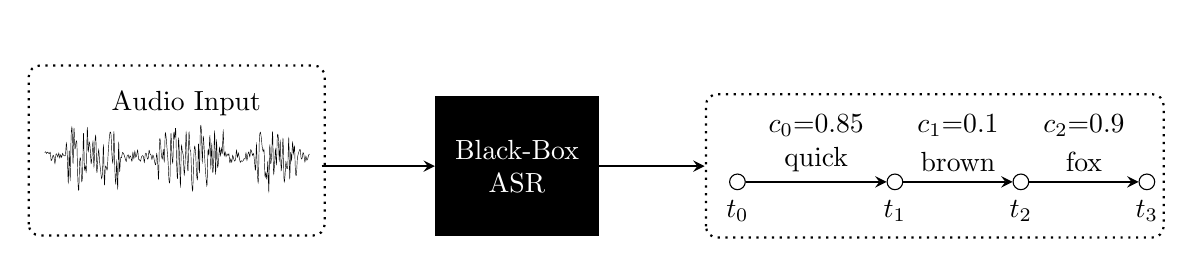
\begin{tikzpicture}[scale=0.4, samples=280, domain=0:7*360]
    % Audio Input
    \begin{axis}[
        width=10cm, height=4cm,
        enlarge x limits=false,
        xtick=\empty,
        axis lines*=middle,
        hide x axis,
        hide y axis
    ]
    \addplot [no markers, smooth] { (sin(3*x)+rand*2) * (x < 200) + (3*sin(3*x)+rand*10) * and(x > 200, x < 720) + (sin(3*x)+rand*2) * and(x > 720, x < 1080) + (3*sin(3*x)+rand*10) * and(x > 1080, x < 1700) + (sin(3*x)+rand*2) * and(x > 1700, x < 2000) + (3*sin(3*x)+rand*10) * and(x > 2000, x < 2400) + (sin(3*x)+rand*2) * (x > 2400)};
    \end{axis}
    \node[invisNode, minimum size=20pt] (h0) at (4.5, 3) {Audio Input};
    \draw[thick,dotted, rounded corners] ($(-0.5,-1.2)$) rectangle ($(h0.north east)+(2.7,-0.5)$);

    % Black-Box ASR
    \node[blackSquareNode] (h2) at (15, 1) {\parbox{2cm}{\centering Black-Box \\ ASR}};

    % Connection audio --> black-box
    \node[invisNode] (h1) at (8.75, 1) {};
	\draw[stateTransition] (h1) to[out=0,in=180] node [midway, sloped, below] {} (h2);

    % One-best sequence with confidence scores
    \node[smallnode] (n1) at (22, 0.5) [label=below:$t_0$]{};
    \node[smallnode] (n2) at (27, 0.5) [label=below:$t_1$]{};
    \node[smallnode] (n3) at (31, 0.5) [label=below:$t_2$]{};
    \node[smallnode] (n4) at (35, 0.5) [label=below:$t_3$]{};
	\draw[stateTransition] (n1) to[out=0,in=180] node [midway, sloped, above] {quick} (n2);
	\draw[stateTransition] (n2) to[out=0,in=180] node [midway, sloped, above] {brown} (n3);
	\draw[stateTransition] (n3) to[out=0,in=180] node [midway, sloped, above] {fox} (n4);
    \node[invisNode] (c1) at (24.5, 3) [label=below:$c_{0}{=}0.85$]{};
    \node[invisNode] (c2) at (29, 3) [label=below:$c_{1}{=}0.1$]{};
    \node[invisNode] (c3) at (33, 3) [label=below:$c_{2}{=}0.9$]{};
    \draw[thick,dotted, rounded corners] ($(n1.south)+(-1,-1.5)$) rectangle ($(c3.north east)+(2.5,0.25)$);

    % Black-box --> word sequence
    \node[invisNode] (h3) at (21, 1) {};
	\draw[stateTransition] (h2) to[out=0,in=180] node [midway, sloped, below] {} (h3);
	

\end{tikzpicture}

\end{document}